\documentclass[a4paper,12pt]{article}
\usepackage[left=1cm,right=1cm,top=3cm,bottom=3cm,a4paper]{geometry}
\usepackage{amsmath}
\usepackage[pdftex]{graphicx}
\usepackage{graphicx}
\usepackage{kotex}
\usepackage[onehalfspacing]{setspace}
\begin{document}
	\begin{flushleft}
		$<$Joule-Thomson effect and molecular forces `*Reif 5.10절$>$ 
	\end{flushleft}
\paragraph{줄-톰슨 효과와 분자간 힘}
이상기체의 경우 
$$\left. \frac{T}{V}\frac{\partial V}{\partial T} \right)_p=\frac{T}{V}\frac{Nk_B}{P}=1 $$
에서 J-T coefficient가 0이다. 즉, 이상기체는 압력을 바꿔준다고 해서 온도가 변하지 않는다. 따라서 free expansion이나 throttling process는 실제 기체들에게만 의미있는 과정이다.
실제 기체의 상태방정식은 다음과 같이 나타낼 수 있는데,
$$p=k_BT(n+B_2(T)n^2+B_3(T)n^3+\cdots) \quad \mbox{where }n\equiv N/V \mbox{ (단위부피당 분자수)}$$
위와 같은 표현을  `virial expansion'이라고 부르고, $B_2,B_3,\cdots$ 들을 `virial coefficient'라고 한다. 특별히 이상기체의 경우, 이 virial coefficient가 전부 0이어야 한다.(해보면 금방 알 수 있다.) Virial expansion에서 $n$에 대한 이차항까지만 살리면,   
$$p=\frac{N}{V}k_BT\left(1+\frac{N}{V}B_2(T) \right) $$가 된다. 여기서 $B_2$의 의미는 무엇일까\\
기체 분자는 서로 멀리 떨어져 있을 때 약하게 서로를 당기고(weak long-range attraction) 너무 가까이 있을 땐 강하게 서로를 밀친다(strong short-range repulsion interaction).
\begin{figure}[h]
	\centering
	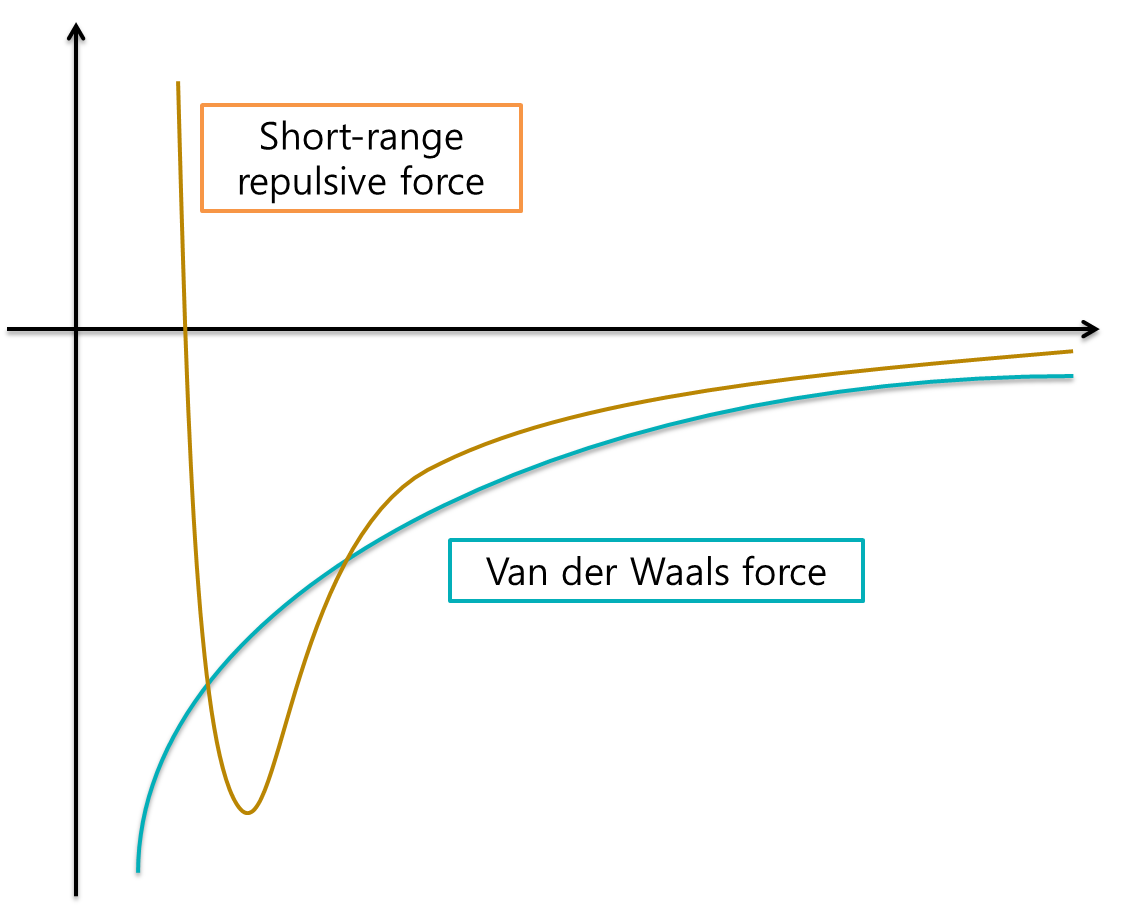
\includegraphics[width=0.5\columnwidth]{repulsive.png}
	\caption{molecular force}
\end{figure}\\
낮은 온도에서는 분자의 운동에너지가 작기 때문에 상대적으로 weak long-range attraction이 우세해진다. 이 경우 분자들이 서로를 약하게 당기기 때문에 이상기체의 경우와 비교해서 기체의 압력이 조금 줄어드는 효과를 보여준다. 즉 $(1+NB_2/V)$ 부분이 1보다 작아져야 하므로 낮은 온도에서의 $B_2(T)$는 음수일 것으로 예측 가능하다.\\
반면 높은 온도에서는 분자의 운동에너지가 weak long-range attraction에 비해서 매우 커지므로 이 효과는 무시할 수 있게된다. 이 경우 분자간 힘에는 strong short-range repulsion이 우세해서 이상기체와 비교했을 때 압력이 증가하는 효과를 보인다. 따라서 $(1+NB_2/V)$ 부분이 1보다 커져야 하므로 높은 온도에서의 $B_2(T)$는 양수일 것이다. 
\begin{figure}[h]
	\centering
	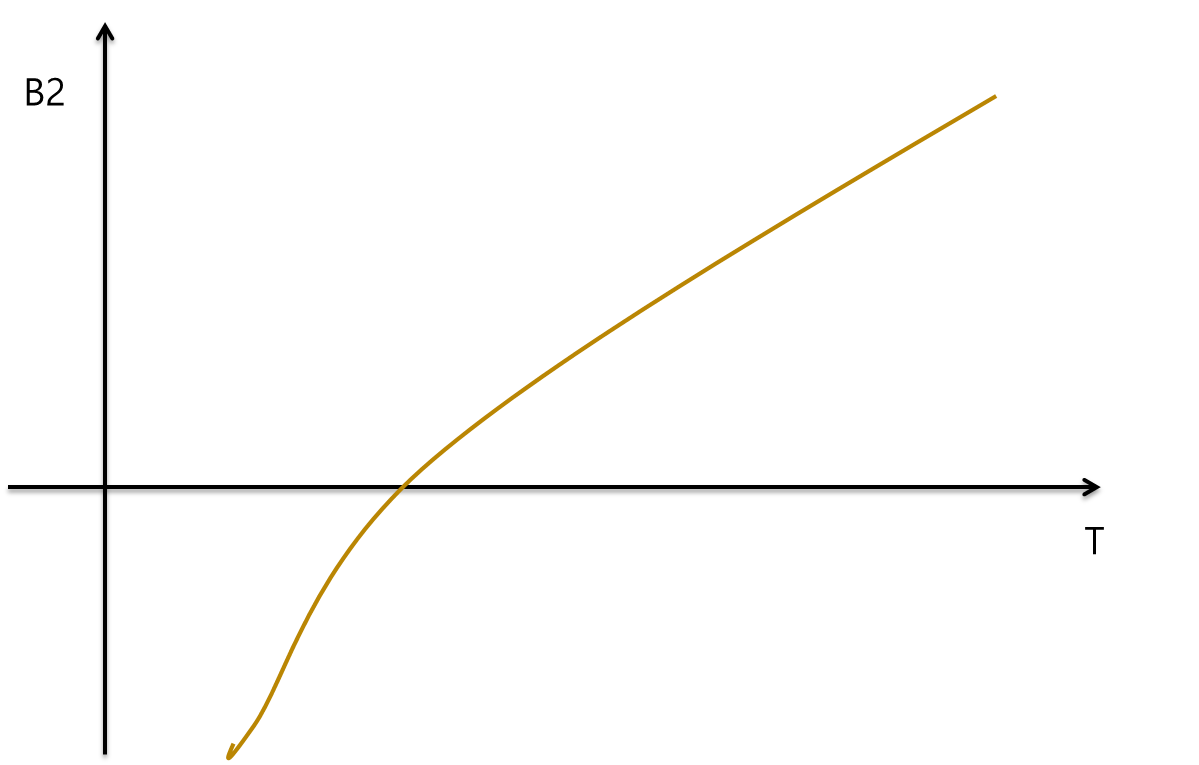
\includegraphics[width=0.5\columnwidth]{B2.png}
	\caption{$B_2$-example}
\end{figure}\\
이제 virial coefficient $B_2$에 대한 논의를 바탕으로 J-T 효과를 설명해보자. J-T coefficient에 대한 식은 다음과 같다.
$$\mu=\frac{1}{C_p}\left(T\left( \frac{\partial V}{\partial T}\right)_p-V  \right) $$
2차항까지만 살린 virial expansion은 
$$p=\frac{Nk_BT}{V}\left(1+\frac{N}{V}B_2 \right)=\frac{Nk_BT}{V}\left(1+\frac{p}{k_BT}B_2 \right)=\frac{N}{V}(k_BT+pB_2) $$
즉,
$$V=N\left(\frac{k_BT}{p}+B_2 \right) $$
따라서 J-T coefficient는
$$\mu=\frac{1}{C_p}\left(T\left( \frac{\partial V}{\partial T}\right)_p-V  \right)=\frac{1}{C_p}\left[T\left( \frac{Nk_B}{p}+N\frac{\partial B_2}{\partial T}\right)-N\left(\frac{k_BT}{p}+B_2 \right)   \right]  $$
$$=\frac{N}{C_p}\left(T\frac{\partial B_2}{\partial T}-B_2 \right) $$
Figure 2에서도 볼 수 있듯이 $B_2$의 $T$에 대한 기울기는 항상 양수이다. 온도가 낮아서 long-range attraction이 우세할 때 $B_2$는 음수가 되고 따라서 $\mu$는 양수가 된다. 온도가 충분히 높아져서 short-range repulsion이 우세할 때는 $B_2>0$ 이기 때문에 $\mu$가 0을 거쳐서 음수로 향한다. 반전곡선(inversion curve)는 attraction과 repulsion 둘의 관계가 뒤치닥거리면서 일어난 결과다. (~ the competing effects between molecular attracton and repulsion) 
\end{document}